%!TEX program = xelatex
% 完整编译: xelatex -> biber/bibtex -> xelatex -> xelatex
\documentclass[lang=cn,11pt,a4paper]{elegantpaper}

\title{科研方法入门(计算机领域)}
\author{徐淑浩
 % \and
 }
\institute{\href{https://faculty.xidian.edu.cn/JT/zh_CN/index.htm}{数据安全特别兴趣小组(DSSIG)}}

\version{1.0}
% \date{\zhtoday}
\date{2022年5月8日}


% 本文档命令
\usepackage{array}
\newcommand{\ccr}[1]{\makecell{{\color{#1}\rule{1cm}{1cm}}}}

\begin{document}

\maketitle

\section{引言}
什么是科研?Research!
科学研究是一个包括调查、收集、整理信息,解释信息、提出疑问、找出不足,思考、进行创新,实验验证、形成论文的系统的过程,所以科研的第一步就是调研、检索现有论文,即Search and re-search。

本文主要介绍科研前论文的检索方法、以及科研时可能用到的工具与资料。
注意,本文优先适用于“数据安全特别兴趣小组(DSSIG)”。
本文使用复旦大学Ethan DENG提供的\href{https://github.com/ElegantLaTeX/ElegantPaper/}{ElegantPaper模板}。

\section{常见名词及概念}
\textbf{(1) 四大安全会议}
\begin{itemize}
  \item ACM Conference on Computer and Communications Security,简称CCS。
  \item IEEE Symposium on Security and Privacy,简称S\&P。
  \item Usenix Security Symposium,简称USENIX Security。
  \item ISOC Network and Distributed System Security Symposium,简称NDSS。
\end{itemize}

\textbf{(2)三大密码学会议}
\begin{itemize}
  \item International Cryptology Conference,简称CRYPTO(美密)。
  \item European Cryptology Conference,EUROCRYPT(欧密)。
  \item Annual International Conference on the Theory and Application of Cryptology and Information Security,ASIACRYPT(亚密)。
\end{itemize}

\textbf{(3)JCR分区与中科院分区}是论文的不同分区方式,其划分标准略有差异,前者是由Clarivate Analytics公司制定,后者由中国科学院国家图书馆制定。

\textbf{(4)四大论文出版社}:IEEE、ACM、Springer、Elsevier。

\textbf{(5)DOI}(Digital Object Identifier)是由国际标准化组织(ISO)标准化的用于唯一标识对象的持久标识符或者句柄,不仅仅论文有,其他的发表物或者其他的东西也有DOI,通过这个DOI可以找到对应的论文。

\section{检索方法与检索工具}
\subsection{CCF推荐期刊和会议}
% \href{https://www.ccf.org.cn/Academic_Evaluation/By_category/}{https://www.ccf.org.cn/Academic_Evaluation/By_category/}
\href{https://www.ccf.org.cn/Academic_Evaluation/By_category/}{《中国计算机学会推荐国际学术会议和期刊目录》},
是由中国计算机协会(CCF)提出的一个值得计算机界研究者们发表研究成果的推荐列表,其中推荐期刊和会议包含A、B、C三个等级,与JCR分区无关。

以其中的“网络与信息安全”领域为例,推荐学术刊物中,TDSC、TIFS和Journal of Cryptology为三个A类期刊,后面给出了此期刊在dblp上的目录网址。
一般来说,老师建议认真阅读A类期刊论文和A、B类会议论文,通常会议论文实时性相对更好,基本是今年投稿的论文今年就会发表,而期刊实时性较差,有时候一篇论文要3年才可以检索到。
人工智能、计算机视觉和机器学习方向同学一般关注“人工智能”这个领域。

\subsection{DBLP}
\href{https://dblp.org/}{DBLP}是一个计算机科学文献目录网站。
既然《中国计算机学会推荐国际学术会议和期刊目录》中给的网址也是DBLP网站的,那我们首先介绍DBLP。
我们可以通过这个网站检索论文、下载论文的引用,而查看、下载论文则会转到论文的原出版社。
\begin{figure}[!htb]
\centering
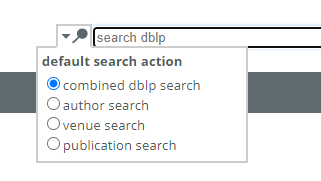
\includegraphics[width=0.5\textwidth]{SecarchInDblp.png}
\caption{}
\label{fig.search_in_dblp}
\end{figure}

\textbf{检索}。
最简单的检索方式就是在搜索框输入论文名字进行检索。
如\figref{fig.search_in_dblp}所示,在搜索框的左边可以选择检索的方式,包含作者搜索、venue(地点)搜索、发表物搜索、混合搜索,默认是混合搜索,但是其中的发表物搜索和我想象的不一样,大家可以试一下。

大家都知道,很多搜索引擎都是支持高级搜索的,通过高级搜索的方式可以使检索内容更加精准。
DBLP也支持通过搜索语句搜索,这类的搜索引擎一般支持的检索语句规则都比较简单。
\begin{enumerate}
  \item 关键词不区分大小写,且为前缀匹配;
  \item 使用\$(美元)符号取消前缀匹配,变成精确匹配;
  \item 使用空格表示逻辑与;
  \item 使用管道符号 $|$ 表示逻辑或。
\end{enumerate}
注意:当给定多个关键词(以空格分隔)时,只有所有的词都满足时才会匹配,所以不确定的词只放确定前缀即可。

\textbf{期刊或者论文目录}。
我们可以通过CCF推荐会议/期刊网站进入查看某个期刊或会议论文的目录,也可以直接在dblp中搜索进入,以\href{https://dblp.uni-trier.de/db/conf/ccs/index.html}{CSS}为例。
最上面是“workshop”,有时候会议的workshop中的论文并不属于主会论文,往下翻我们可以看到列出了每年会议的时间地点,可以点击“contents”或点击左边的“view”进入某一年的目录。

以2020年为例,分为很多session,每个session对应一个主题。
我们可以找到自己感兴趣的论文,点击右侧的view - electronic edition via DOI,到这篇论文的出版方查看论文的详细信息。
由于CCS是ACM的会议,所以会重定向到ACM网站中显示此会议的此篇论文。
而CCS原本就是由ACM出版,所以我们也可以从ACM网站看到CCS'20的论文\href{https://dl.acm.org/doi/proceedings/10.1145/3320269}{目录}。

\begin{figure}[!htb]
\centering
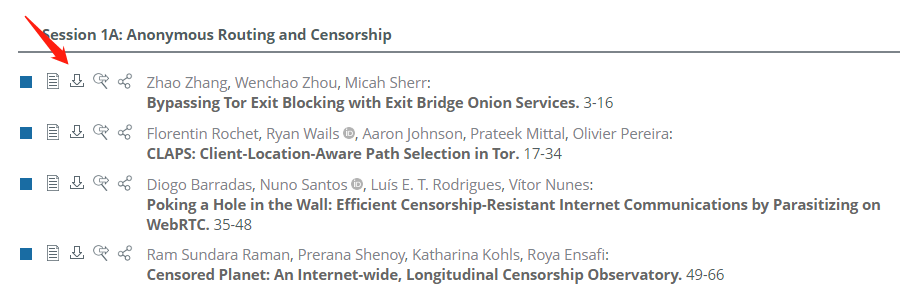
\includegraphics[width=0.8\textwidth]{ccs20_1a.jpg}
\caption{}
\label{fig.ccs20_1a}
\end{figure}
\textbf{引用下载}。
使用latex撰写论文时需要使用到论文的bib引用,而一般dblp中对bib格式整理的相对标准,不会出现问题,所以很多时候可以直接在dblp中拷贝某论文的bib。
如\figref{fig.ccs20_1a}所示,以CCS'20中Session 1A的第一篇论文为例,我们指向红色箭头所指的按钮,选择BibTex就会进入bib页面如\figref{fig.ccs20_bib}。
点击复制即可,注意红色箭头所指的位置可以调整bib文件的格式,一般情况下选择Condensed即可。
\begin{figure}[!htb]
\centering
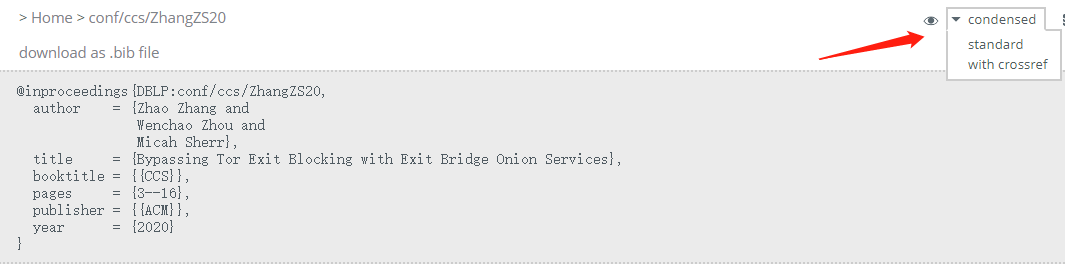
\includegraphics[width=0.98\textwidth]{BibDownload.jpg}
\caption{}
\label{fig.ccs20_bib}
\end{figure}

\textbf{插件}。
因为CCF推荐的期刊或会议很多,有时候找到论文不确定是不是值得看,挨个在ccf推荐里找很慢,所以可以使用浏览器插件“CCFrank”。
此插件目前可以在Google浏览器“chrome 网上应用店”中可以搜索安装,支持在 dblp 和 Google 学术的搜索结果中显示中国计算机学会(CCF)推荐的国际会议和期刊排名。

\subsection{其它检索工具推荐}
\textbf{(1)\href{https://www.webofscience.com/wos/alldb/basic-search}{Web of Science}}(WoS,原称~Web of Knowledge),最初由~Institute for Scientific Information(ISI)组织创建,目前由属于~Clarivate~公司。
它收录了自然科学、工程技术、生物医学等各个研究领域最具影响力的超过8700多种核心学术期刊。
利用Web of Science 丰富而强大的检索功能--普通检索、被引文献检索、化学结构检索,您可以方便快速地找到有价值的科研信息,既可以越查越旧,也可以越查越新,全面了解有关某一学科、某一课题的研究信息\footnote{引用自“百度百科”}。

\begin{figure}[!htb]
\centering
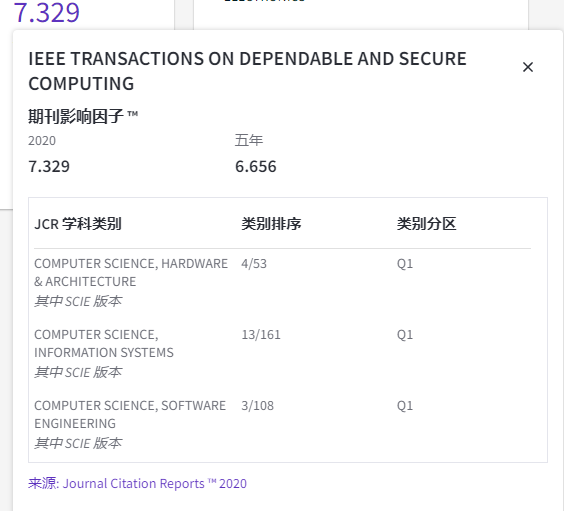
\includegraphics[width=0.6\textwidth]{tdsc22_IF.jpg}
\caption{}
\label{fig.tdsc22_IF}
\end{figure}
最开始,有些论文的质量不确定时,我就会在这个网站查看一下。
我们以2022年TDSC中的第一篇论文《Verifying and Monitoring IoTs Network Behavior Using MUD Profiles》为例,进入详情界面我们可以查看期刊影响力如\figref{fig.tdsc22_IF},包括影响因子和~JCR~分区。
% JCR分区也是衡量一个期刊好坏的标准。
也可以查看这篇论文的引用和被引用等。
当然,这个网站以及后面要讲的网站及工具不仅仅只有这么一点作用,我讲到的只是冰山一角,更多的用处和使用技巧需要大家一起探索并分享。

\textbf{(2)\href{https://sci-hub.shop/}{SCI-HUB}}是世界上第一个向大众和公众提供数千万科研论文访问的prate(翻印)网站。用的不多,不多做介绍。\href{https://s1.sci-hub.org.cn/}{SCI-HUB的CN网站}。

\textbf{(3)\href{https://scholar.google.com/}{Google Scholar}},谷歌学术。
谷歌学术应该是最全面的搜索引擎,功能也齐全,支持引文中检索和多版本检索。
注意,在这些网站(不仅仅是谷歌学术)上一般都会有作者的主页,而谷歌学术的作者主页汇总的比较全面,也可以关注作者,看作者的最新研究进展。
国内可以使用谷歌学术镜像网站,数据基本是同步的。

\textbf{(4)四大出版社网站}。
\href{https://ieeexplore.ieee.org/Xplore/home.jsp}{IEEE Xplore}、\href{https://dl.acm.org/}{ACM DL}、\href{https://link.springer.com/}{Springer}、\href{https://www.sciencedirect.com/}{Science Direct}也提供对应的论文检索功能。

\textbf{(5)\href{https://www.cnki.net/
}{中国知网}}。

\section{科研开始与科研资料推荐}
\subsection{科研开始}
讲了这么多检索方法,相信大家已经跃跃欲试了(>﹏<)。
那么如何开始呢?

刚接触一个领域,想快速的了解这个领域的研究现状,可以先找一篇综述性文章,或者某篇文章的综述(related work)部分。
检索综述类论文时,可以带上关键字study、survey、review等,这三个是最常见的表明是综述类文章的关键字。
注意综述类文章要求尽量的新,最好是近一年的,而综述类文章不需要必须是上面讲到的A、B类会议或A类期刊。

那有小部分聪明的同学又要问了,“我都不知道我的方向该用什么关键字,尤其是英文我更不知道怎么翻译,那我如何正确地输入关键字检索呢?”
确实,有时候我们发现,直接告诉你一个研究方向也未必自己可以找到合适的论文。
如果我们一点也不知道该用什么单词去检索,可以去知网等查找下中文的论文,在其中的英文摘要或者参考文献中找一下。

如果导师已经给你一篇文章,那么我们可以从这篇文章入手。
既然是导师给你的文章,必定是有一定的代表性,或者比较有价值。
我们首先需要认真阅读这篇文章,把该理解的部分一定要理解,最开始读论文,理解思想最关键,至于一些实在看不懂的公式或者技术可以先作为“黑盒”处理,以后再搞明白。
其中的综述(related work)部分认真阅读并理清楚此作者对其它论文及研究现状的评价,然后积累其中的关键词,用于我们检索论文。
\textit{一旦你找到了这件“毛衣的第一个线头”,后面思路自然就会打开了。}
当论文中引用了其他论文中的技术时,在需要弄懂的时候,递归的搞明白。

\begin{figure}[!htb]
\centering
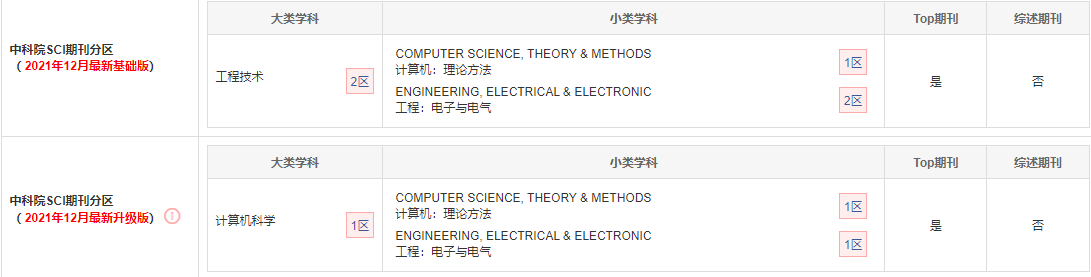
\includegraphics[width=0.9\textwidth]{tifs_zky.jpg}
\caption{}
\label{fig.tifs_zky}
\end{figure}
对于SCI期刊可以根据分区确定期刊质量,上面提到了~Web of Science~可以查看JCR分区,国内一般以中科院分区为标准。
有很多网站可以查到期刊的中科院分区,例如\href{http://www.letpub.com.cn/index.php?page=journalapp}{LetPub}
以TIFS为例,其分区结果如\figref{fig.tifs_zky}。
学校\footnote{此处仅指西安电子科技大学}认定一般是按照大类分区,我们可以看到TIFS在2020年12月升级版的中科院SCI分区中,大类属于计算机科学,且TIFS是1区,且属于顶刊。
当然SCI分区并不能完全代表论文的质量,需要看这个期刊在业界(尤其是小方向)的口碑。

\subsection{资料推荐}
\begin{itemize}
  \item 《Science Research Writing》:由~Hilary Glasman-Deal~编写的针对非英语母语科研人员的科研写作指导书。书中介绍了进行科研写作时每一部分推荐的用词、句式、结构,纯英文版,但是不是很难读。\textcolor{red}{必看}
  \item 《Introduction to Modern Cryptography》:由~Jonathan Katz~等人编写的现代密码学介绍,优先推荐密码理论方向的同学学习。其中的概念和专业术语特别的多,极其难阅读,此版本是纯英文版,纯英文版的好处在于写英文论文时便于查找一些术语。国内有翻译版本,但基本是直译,不太容易理解。
  \item 《现代密码学理论与实践》:由~Wenbo Mao~著,王继林等译,英文原版名为《Modern Cryptography: Theory and Practice》。优先推荐做安全协议方向的同学阅读。
  \item 《机器学习》:周志华教授著,又名“西瓜书”,因为其全书基本以西瓜为例而的名。西瓜书是机器学习领域经典入门书籍,优先推荐机器学习、深度学习方向同学阅读学习,其中有大量的公式推导,有一定的阅读难度。周老师为了尽可能多的让读者通过西瓜书对机器学习有所了解,所以在书中对部分公式的推导细节没有详述,但是这对那些想深究公式推导细节的读者来说可能“不太友好”\footnote{引用自南瓜书}。所以推荐与《南瓜书——Pumpkin Book》配合使用。南瓜书的最佳使用方法是以西瓜书为主线,遇到自己推导不出来或者看不懂的公式时再来查阅南瓜书
  \item 《Deep Learning——深度学习》:美国 Ian Goodfellow 等人著,人工智能领域的“圣经”,优先推荐人工智能、深度学习方向的同学阅读。
\end{itemize}

以上所推荐的书籍,在本组的网站/群中均有电子版本,我也将其上传到了\href{https://pan.baidu.com/s/1Z-PE5qZdd7RmlNwIYpFNtQ 
}{我的网盘}中,提取码:c704。

\section{论文“副产品”的检索}
一篇论文一般会伴随有很多其它的“副产品”,比如此篇论文的实现源码、系统,论文的其他版本、会议论文的报告PPT和视频。
以USENIX Security为例,其上的所有论文,在其官网上都可以下载到报告PPT以和报告视频,如\figref{fig.UsenixExample}所示。
\begin{figure}[!htb]
\centering
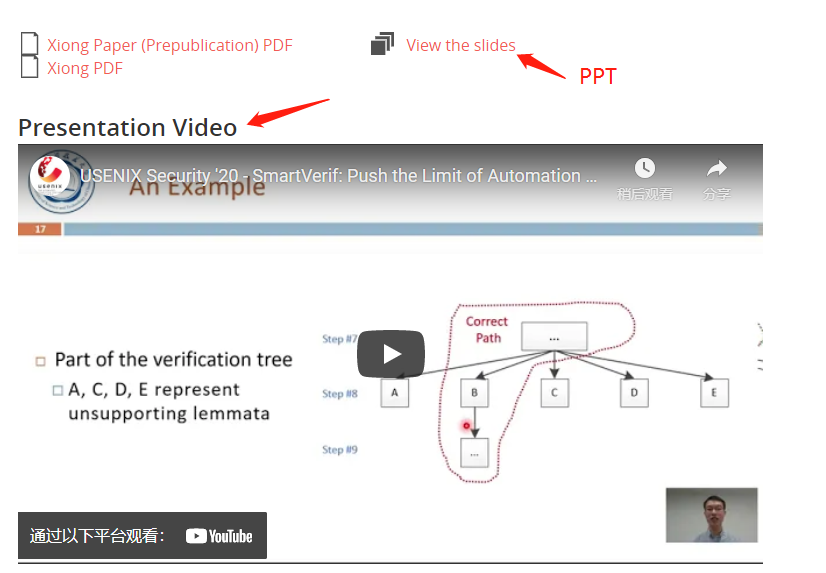
\includegraphics[width=0.98\textwidth]{UsenixExample.png}
\caption{}
\label{fig.UsenixExample}
\end{figure}

有些论文在刚写完后会将其托管到一些网站(比如~arXiv~和~ePrint~),申明论文的著作权,保护自己的知识产权。
还有一个重要的原因,有时候期刊或者会议有页数限制,无法完全的展示,就会在这些网站上放完整版本。
当然还有其他的版本,如作者的博客中的版本,这些版本论文对细节的描述往往更全面,更容易理解。
所以对于某些必须要看懂却看不懂的论文找到其它版本还是很有用的。

论文的源码。当我们看完某篇论文想要复现时,如果有论文的源码是再好不过的了。当然并不是所有的论文都会公开源代码,更不是所有的论文都有源代码。
针对有源码的论文,我们该如何查找呢?大约从两个方向查找:Github、作者的主页(如果是高校老师,可以是学校的教师主页,个人博客主页)。当然Github最开始也是按照作者的名字找其Github主页,看一下其~repository~目录中是否有,也可以直接检索论文名字或者论文中系统的名字。其次是去~Google~上,查找作者的资料,试图找到其主页,找到主页后可以看是否有源码。
当然,就算作者不给源码,有时我们也可以找到其他人复现此论文的源码,也可以作为参考。

数据集。推荐一个查找数据集的网站 Google 的\href{https://datasetsearch.research.google.com/}{~Dataset Search~}这个用的不是很多,但是感觉还不错。

\section{论文写作}
\subsection{\LaTeX}
本节基于个人CSDN博文\href{https://blog.csdn.net/qq_40115871/article/details/105901765}{LaTeX与Sublime Text环境搭建 -扫雷篇}。
论文优先推荐使用~Latex~撰写,\LaTeX 是一种~TEX~排版系统,作者能够使用预定义格式以达到高质量排版。LaTeX的发行版有很多,常见的有TeX Live、MikTeX等。

\textbf{(1)如何选择LeTeX 版本}。
由于本人开始也是迷茫该如何选择,故看过一篇资料,\href{https://zhuanlan.zhihu.com/p/45174503}{[LaTeX 发行版] 2018年,为什么不推荐使用 CTeX 套装了}。
总体来说,Tex Live~目前使用范围略广,自己毕业论文的模板也是~Tex Live的,自己的使用感受也不错。

\begin{figure}[!htb]
\centering
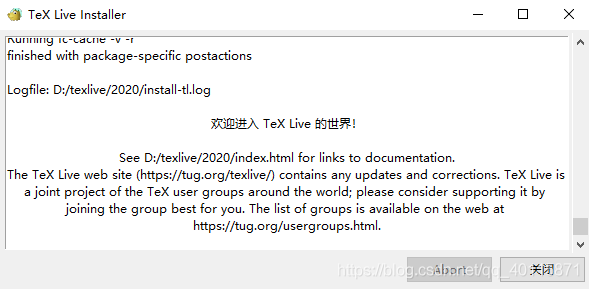
\includegraphics[width=0.78\textwidth]{LatexInstall.png}
\caption{}
\label{fig.LatexInstall}
\end{figure}
\textbf{(2)安装TexLive}。
不建议采用在线安装方式,建议先下载镜像ISO文件后安装,\href{http://tug.org/texlive/}{tug下载链接}。
下载完之后是个ISO镜像文件,运行里面的install-tl-windows.bat即可安装,安装完成的界面如\figref{fig.LatexInstall}所示。
安装完这时候我们就可以使用LaTeX了,在开始菜单里找到新安装的TeX Live目录,目录下有一个TeXworks editor。这是由于我们安装时选择了默认安装,默认安装了~Texworks~前端。
但是~Texworks~是没有代码/命令提示的,而且据说 Bug 很多,“安逸派”可以选择安装 TeXstudio。
如果着急使用,或者不在乎颜值啥的,到这里就算是安装完成了。但是对于某些完美主义者、或者感觉~TeXworks/TeXstudio~界面太难看,那么我们可以把它配置到~Sublime Text~中。

\textbf{(3)安装Sublime Text}。对于程序员们来说,Sublime Text并不陌生,它算是一个文本或者代码编辑器吧,只有几十M的大小,打开迅速,而且其中含有丰富的插件,可以将其打造得高大上。对于Sublime Text的夸赞,这里就不多说了。

下载网址\href{http://www.sublimetext.com/3}{Download - Sublime Text},对于有便携版的软件我一般是推荐使用便携版(portable version),因为便携版不需要安装,而且我们装的插件啊,进行的配置都保存在软件主目录下,这样我们要是换了电脑,或者电脑重装了,我们只需要把整个文件夹备份一下可以继续使用。

便携版下载完之后,解压,点击目录下的“sublime\_text.exe”即可使用,Sublime Text不是免费的,可以无限期是用,但是会提醒注册且一直显示未注册。


\textbf{(4)配置Sublime Text}。
\begin{enumerate}
  \item 自动安装Package Control插件。使用快捷键\lstinline{Ctrl + `} (这个是数字1左边的那个键)或者点击View - Show Console打开控制台。输入如下代码:
  \begin{lstlisting}
  import urllib.request,os; 
  pf = 'Package Control.sublime-package'; 
  ipp = sublime.installed_packages_path(); 
  urllib.request.install_opener( urllib.request.build_opener( urllib.request.ProxyHandler()) ); 
  open(os.path.join(ipp, pf), 'wb').write(urllib.request.urlopen( 'http://sublime.wbond.net/' + pf.replace(' ','%20')).read())
  \end{lstlisting}
  或者如下代码:
  \begin{lstlisting}
  import urllib.request,os,hashlib; h = '6f4c264a24d933ce70df5dedcf1dcaee' + 'ebe013ee18cced0ef93d5f746d80ef60'; pf = 'Package Control.sublime-package'; ipp  = sublime.installed_packages_path(); urllib.request.install_opener( urllib.request.build_opener( urllib.request.ProxyHandler()) ); by = urllib.request.urlopen( 'http://packagecontrol.io/' + pf.replace(' ', '%20')).read(); dh = hashlib.sha256(by).hexdigest(); print('Error validating download (got %s instead of %s), please try           manual install' % (dh, h)) if dh != h else open(os.path.join( ipp, pf), 'wb' ).write(by)
  \end{lstlisting}
  (这两组代码是自己查到的)然后按回车,这是自动安装方法。但是这里大概率会出问题,因为自己两次都出了问题,有可能是由于墙的原因吧。
  \item 手动安装Package Control插件,如果上面安装成功请忽略这一段。
  首先下载 \href{https://sublime.wbond.net/Package}{Package Control.sublime-package},但是这个下载也超级慢,我把它放在了\href{https://pan.baidu.com/s/1hGTMVhRqANAJREAMJhse_A}{百度云盘},提取码:pgj8 。
  下载完后打开sublime text 3,点击Preferences - Browse Packages...,会打开一个目录,然后回到上一级目录,有个Installed Packages文件夹,打开这个文件夹,将我们下载下来的Package Control.sublime-package文件拷贝到该文件夹下,如果里面有一个了就替换它(这个应该是刚才我们自动方式下载的,但是没成功)。然后重启Sublime Text,观察 Preferences菜单下是否出现了Package Settings和Package Control,如果有的话就说明安装成功了。这时我们就可以打开Sublime Text的另一扇大门了,使用快捷键\lstinline{Ctrl + Shift + P},再输入install,选择install package,想安装什么插件,直接搜索就好了。

  \item 安装LaTeXTools插件。使用快捷键\lstinline{Ctrl + Shift + P}打开Package Control,输入Install Package命令,加载完仓库再输入LaTeXTools进行安装,这是可以看见左下角会显示正在安装。稍等后会出现\figref{fig.LatexTools}的文档,表示安装成功。但是我第一安装的时候就出现了安装失败的情况,具体的报错信息没有记录,但是大体的解决过程是把安装LaTeXTools的插件都单独下载并放到了打开的Packages文件夹下,但是我后来的两次安装都没有出现这种情况,还是建议换换网络多试几次,手动方式太麻烦。
\begin{figure}[!htb]
\centering
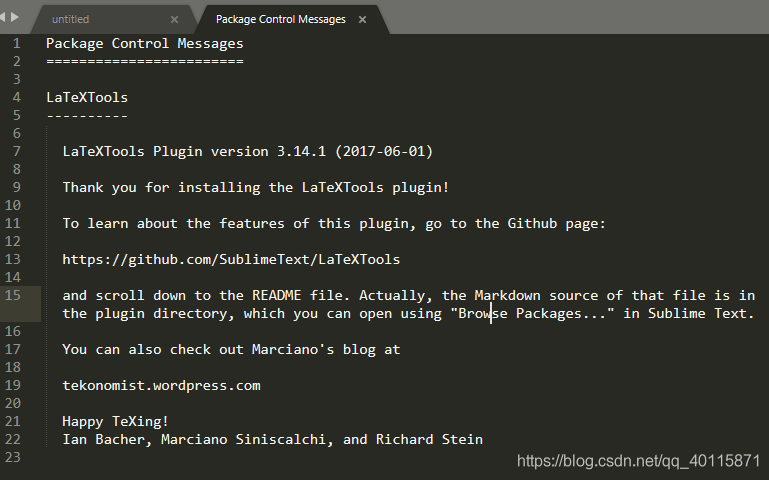
\includegraphics[width=0.78\textwidth]{LatexTools.png}
\caption{}
\label{fig.LatexTools}
\end{figure}

  \item 配置LaTeXTools插件。点击Preferences - Browse Packages,打开“LaTeXTools”文件夹,将LaTeXTools.sublime-settings文件复制到上一级目录(也就是刚打开的目录)的User目录下。然后打开LaTeXTools.sublime-settings文件如\figref{fig.ConfigLatexTools}所示,1)首先找到Platform settings: adapt as needed for your machine下的"windows"下的"texpath",texlive安装路径$\backslash \backslash$ 年份 $\backslash \backslash$ bin $\backslash \backslash$ win32; \$PATH。再把"distro"后更改为"texlive"。2)在找到Build engine settings部分下的"builder": "traditional"(应该在386行)修改为"builder": "simple"。\footnote{详见\href{https://github.com/SublimeText/LaTeXTools}{Github}}
\begin{figure}[!htb]
\centering
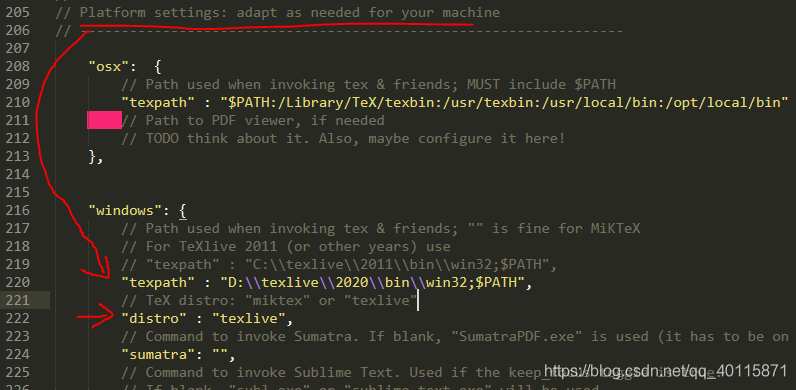
\includegraphics[width=0.85\textwidth]{ConfigLatexTools.png}
\caption{}
\label{fig.ConfigLatexTools}
\end{figure}

\end{enumerate}

\textbf{(5)下载并配置Sumatra PDF}。
Sumatra PDF可以在其\href{http://www.sumatrapdfreader.org/download-free-pdf-viewer.html}{官网}下载并安装。然后将Sumatra PDF安装目录配置到path环境变量中,默认情况下是C:$\backslash$Program Files$\backslash$SumatraPDF。

随便找一个LaTeX模板,然后用Sublime Text打开,使用快捷键\lstinline{Ctrl + Shift +b}选择LaTeX - PdfLaTeX,等编译之后就会自动打开Sumatra PDF显示模板。
然后我们需要配置反向解析,反向解析就是在PDF中的某个位置按住Ctrl单击或双击可以找到对应代码中的位置,方便改错误,自带的Texworks前端是有反向解析的。在打开的Sumatra PDF左上角点击三条杠的按钮 - 设置 - 选项,就会弹出对话框。
修改“设置反向搜索命令行”下的命令,在文本框中填入:
\begin{lstlisting}
"Sublime Text Path\sublime_text.exe" "%f:%l"
\end{lstlisting}
比如我的安装路径是\lstinline{D:\Program Files\Sublime Text Build 3211 x64},那么我填的结果如\figref{fig.ConfigSumatra}(前面的路径显示不开了)。
\begin{figure}[!htb]
\centering
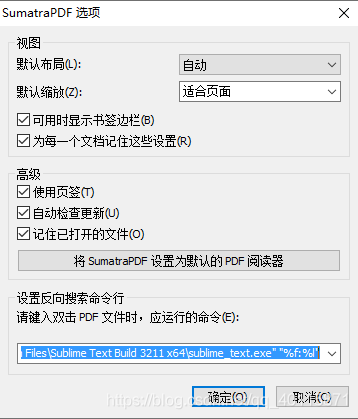
\includegraphics[width=0.5\textwidth]{ConfigSumatra.png}
\caption{}
\label{fig.ConfigSumatra}
\end{figure}

\textbf{(6)安装LaTeXYZ}。
装完环境之后发现,使用Sublime Text还是没有使用Texworks那样好用,原因是没有代码提示。我们只需要给Sublime Text再装一个LaTeXYZ插件就可以实现代码提示功能。像之前一样,使用组合键\lstinline{ctrl + shift + P},输入Install Package回车之后输入LaTeXYZ,搜索到此插件后点击安装即可。

\subsection{论文模板下载}
大部分外文论文出版社都提供Latex模板,我们只需要下载并使用即可。
而模板首先可以通过会议或期刊的出版社的“作者”网站下载,如\href{https://ieeeauthorcenter.ieee.org/}{IEEE}、\href{https://www.springer.com/cn/computer-science/lncs/conference-proceedings-guidelines}{Springer}和\href{https://www.elsevier.com/authors/policies-and-guidelines/latex-instructions}{Elsevier},而有时会议的模板会在所投递会议的主页给出。
% https://ieeeauthorcenter.ieee.org/
% https://www.springer.com/cn/computer-science/lncs/conference-proceedings-guidelines
% 
% https://www.elsevier.com/authors/policies-and-guidelines/latex-instructions

\section{其它}
推荐一些平时经常可以用到的工具或网站。
\textbf{Gitbub}~真的是一个很好的网站,希望大家可以将其运用起来,在其上面可以找到的东西远不止代码,当然其代码的托管功能也非常的实用。举个例子,著名的深度学习书籍,花书《Deep Learning》的翻译工作也是在~Github~上进行的,\href{https://github.com/exacity/deeplearningbook-chinese}{项目网址},你想找电子版duck不必某度网盘或者CS*N积分下载,在~Github~上就可以下载PDF版。
目前“国产”版的~Github~\href{https://gitee.com/}{Gitee}发展也极其迅速,也推荐大家使用。

\textbf{Markdown}~是一种轻量级标记语言,很容易排版,支持latex公式。有时候我们好不容易在word中利用公式编辑器将公式写完,又需要将其转到latex中,这就很麻烦,所以md中的公式很容易兼容latex。

\textbf{EndNote}功能也很多,但是我把他定位为一个文献管理工具,当阅读或者下载的论文变多之后,自己用文件夹管理就很不方便,那么我推荐使用EndNote管理,分类分组、查看比较方便。

\section{写在最后}
以上方法与经验仅供参考。
众所周知,学习方法总是多种多样的,所以本文仅在给大家提供思路,希望大家从中获得启发,找到属于自己的方法才是本文的最终目的。

全文写完再读来才发现并没有达到想要的目的,这些方法和经验都是自己在摸索中总结出来的,但是有些经验写不出来,只有实践多了才知道,只可意会不可言传,甚至不可意会不可言传。

本文是在自己\href{https://blog.csdn.net/qq_40115871/article/details/115861140}{原CSDN博文}和\href{https://zhuanlan.zhihu.com/p/367339390}{知乎文章}的基础上修改而来,在临毕业之际完成本文,思绪与感慨溢于言表。本文完成的仓促,拙文难免有错误与疏漏,本文已挂载到Gihub和Gitee中,欢迎后续师弟师妹在此基础上修改并完善。

% \subsection{奖学金评定}
% \begin{lstlisting}
% \documentclass[a4paper,11pt]{elegantpaper}
% \end{lstlisting}

% \textbf{注意}:Elegant\LaTeX{} 系列模板已经全部上传至 \href{https://www.overleaf.com/latex/templates/elegantpaper-template/yzghrqjhmmmr}{Overleaf} 上,用户可以在线使用。另外,为了方便国内用户,模板也已经传至\href{https://gitee.com/ElegantLaTeX/ElegantPaper}{码云}。




% \begin{figure}[!htb]
% \centering
% \includegraphics[width=0.9\textwidth]{founder.png}
% \end{figure}


% 如果需要设置为国标 GB7714-2015,需要使用:
% \begin{lstlisting}
%   \documentclass[citestyle=gb7714-2015, bibstyle=gb7714-2015]{elegantpaper} 
% \end{lstlisting}

% 如果需要添加排序方式,可以在导言区加入
% \begin{lstlisting}
%   \ExecuteBibliographyOptions{sorting=ynt}
% \end{lstlisting}

% 启用国标之后,可以加入 \lstinline{sorting=gb7714-2015}。


% \section{使用 newtx 系列字体}

% 如果需要使用原先版本的 \lstinline{newtx} 系列字体,可以通过显示声明数学字体:

% \begin{lstlisting}
% \documentclass[math=newtx]{elegantpaper}
% \end{lstlisting}

\section{致谢}
特别感谢导师姜涛在科研中给予的指导、在生活学习中给予的信任与支持。

\end{document}
